\documentclass[11pt]{asu}

\usepackage[]{graphics}
\usepackage{graphicx}
\usepackage{setspace}
\usepackage{lscape}
\usepackage{rotating}
\usepackage{listings}
\usepackage{url}
\usepackage{courier}
\usepackage{csquotes}
\usepackage{fixltx2e}
\usepackage{xinttools}
\usepackage[]{algorithm2e}
\usepackage[toc,page]{appendix}

\newcounter{bitindex}

\clubpenalty=5000
\widowpenalty=5000
\renewcommand\lstlistlistingname{List of Listings}
\setlength{\belowcaptionskip}{.25in}

%c++ listing box settings
\lstset{language=C++,
	numberstyle=\footnotesize,
	basicstyle=\ttfamily\footnotesize,
	morekeywords={uint8_t, uint16_t, uint32_t, uint64_t},
	numbers=left,
	stepnumber=1,
	frame=single,
	breaklines=true,
  showstringspaces=false
}

%create image of a float showing each bit
\newcommand{\floatimage}[3]{%
  \setlength{\unitlength}{1mm}
  \setlength{\fboxsep}{0mm}
  \begin{picture}(130,16)
    % sign bit
  \put(2,4){\framebox(4,8){#1}}
  % exponent
  \setcounter{bitindex}{1}%
  \xintFor* ##1 in {#2}
  \do
  {\put(\numexpr 2+4*\value{bitindex},4){\framebox(4,8){##1}}%
   \stepcounter{bitindex}}%
  % fraction
  \setcounter{bitindex}{1}%
  \xintFor* ##1 in {#3}
  \do
  {\put(\numexpr 34+4*\value{bitindex},4){\framebox(4,8){##1}}%
   \stepcounter{bitindex}}%
  % upper labels
  \put(0,14){\scriptsize{MSB}}
  \put(126,14){\scriptsize{LSB}}
  %lower labels
  \put(3,0){\scriptsize{S}}
  \put(7,0){\line(0,1){2}}
  \put(7,1){\vector(1,0){8}}
  \put(16,0){\scriptsize{Exponent}}
  \put(37,1){\vector(-1,0){8}}
  \put(37,0){\line(0,1){2}}
  \put(39,0){\line(0,1){2}}
  \put(39,1){\vector(1,0){38}}
  \put(79,0){\scriptsize{Fraction}}
  \put(130,1){\vector(-1,0){38}}
  \put(130,0){\line(0,1){2}}
\end{picture}%
}

%inline code command, using courier font
\newcommand{\code}[1]{\texttt{#1}}

\title{A Portable C++ Framework for the Serialization of Floating-Point Numbers}
\degree{Bachelor of Science}
\department{Computer Science}
\gradmonth{May}
\gradyear{2014}
\author{Michael Crawford}  
\thesischair{Cindy Norris, Ph.D.}
\thesismemberone{E. Frank Barry, M.Sc.}
\thesismembertwo{Dee Parks, Ph.D.}
\deptchair{James Wilkes, Ph.D.}
\dean{Dean}

\begin{document}
	\begin{preliminary}
		\maketitle
        \makecopyright
        \begin{abstract}
 Hello world!
\end{abstract}

		\tableofcontents
        \listoftables
        \listoffigures
        \lstlistoflistings
	\end{preliminary}

	\newlinestretch{2}

		\begin{doublespace}
	    \chapter{Introduction}
\label{chap:introduction}

% Establish a presidence 
Personal computers have been developed to a point where those unfamiliar with computer science theory might conclude there is nothing computers cannot do.
While this is an understandable conclusion, it has been proven that there is a limit to the types of computation our ``classical computers", what we today consider general purpose computers, can perform \cite{linz}.
In the last few decades however, the field of quantum mechanics and quantum computing have advanced to the point where primitive operations are now possible in the quantum sphere.
Just this year Google claimed to acheive ``quantum supremacy" in an experiment in which they performed a computation, using a quantum computer, in under five minutes. 
Google estimated that the same computation would take a state-of-the-art super computer 10,000 years to complete \cite{quantum_supremacy}. 
While quantum computers are not general purpose, they can solve NP-Hard and exponentially complex problems in polynomial time or better \cite{TODO}.
This breakthrough in computability will change the way information is stored, secured, and created.


% State the problem
Currently, encryption protocols ensure the integrity of data and identities are trusted.
One such protocol is the the widly adopted Diffe-Hellman protocol, which relies on the historic difficulty of factoring large prime numbers for security \cite{qc:agi}.
The protocol works by using a public and private key pair for each participating party.
Data encrypted using a key (usually a public key) can then be decrypted using the private key.
For example, a person's public and private keys are mathematically related to their private key, and it requires factoring large prime number to derive the private ky from the public key, which is comutationally infeasible with a classical computer.
Quantum computers however, are able to do this in only polynomial time complexity \cite{doi:10.1137/S0036144598347011}.
This development, combined with the growing power of quantum computers, gives rise to security concerns to the Diffe-Hellman protocol in the future.

% Mention the solution
One such development was the BB84 quantum key distribution protocol.
There are many encryption protocols in use today, such as the Diffe-Hellman key exchange protocol (KEP), each of which provide their own various security measures.
The BB84 protocol allows two parties to co-generate a disposable encryption key which can be used once to encrypt then decrypt data, and be discarded after use.
This type of key is known as a one-time-pad, and it gets its security from being disposable; data patterns are harder to identify the fewer times data is encrypted using a key \cite{TODO}.
The BB84 protocol allows for detection of an eavesdropper durring key generation, allowing both parties to abort the key generation process before any encrypted messages are transmitted \cite{qcftgu}.
This thesis presents a peer to peer simulation of the BB84 quantum quantum KEP, and serves as an introduction to programming in the quantum computing paradigm using simulaqron, a quantum network simulator \cite{simulaqron}.

% Describe the thesis' coontribution to the problem

% Describe the thesis content

Chapter~\ref{chap:background} of the thesis provides background information on encryption protocols, the quantum computation paradigm, and other background information related to the BB84 protocol. 

Chapter~\ref{chap:bb84} details the BB84 protocol in its steps, as well as discusses the guarantees the protocol provides the user.

Chapter~\ref{chap:implementation} describes the library.
This describes not only the documentation for the library but also how it can be used.

Chapter~\ref{chap:conclusion} summarizes this simulator and its potential applications, as well as discussing possible future work to improve upon it.


	    8p\chapter{Preliminaries}
\label{chap:background}

% Describe what we need to understand to move forward
In this chapter, we discuss the preliminaries of encryption and quantum computation, the two ideas key to understanding the BB84 quantum KEP.


\section{Encryption}
Consider two parties, Alice and Bob, trying to communicate through a channel.
If the channel is insucure, a malicious third party, Eve, can listen and eavesdrop on the communication.
Encryption helps to make the communication more secure, by obscuring data such that an eavesdropper cannot gain any information by intercepting communication \cite{encrypt}.

\begin{figure}[htp]
\centering
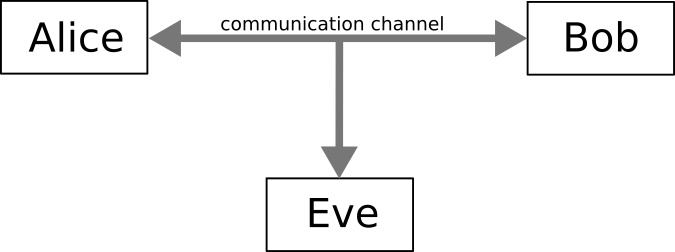
\includegraphics[scale=0.4]{images/classical_communication.png}
\caption{Alice and Bob communicate over an insecure channel with an eavesdropper, Eve}
\label{foo bar}
\end{figure}

In practice, information is encrypted by manipulating the data according to some encryption algorithm.
The goal of a good encryption algorithm is simple: allow the sender and receiver to access the information, but make the data useless to anyone else.
In order to allow for information to be decrypted by the receiver, the algorithm must be reversible with the use of a secret key, also known as the encryption key.
The basic encryption process is as follows:

\begin{itemize}
\item A sender, Alice, composes a message, referred to as the plaintext.
\item Alice encrypts the plaintext into cyphertext using some encryption algorithm and an encryption key.
\item Alice then sends the cyphertext to the receiver, Bob.
\item Bob uses the encryption key to decrypt the cyphertext into plaintext.
\item Note that the plaintext was never transmitted over the network.
\end{itemize}

Encryption appears in two general forms: symmetric and asymmetric, each with their own benefits and drawbacks. 


\subsection{Symmetric Encryption}
% Symmetric Encryption
Symmetric encryption is an encryption method in which both the sender and receiver, Alice and Bob respectively, use the same key.
\begin{figure}[htp]
\centering
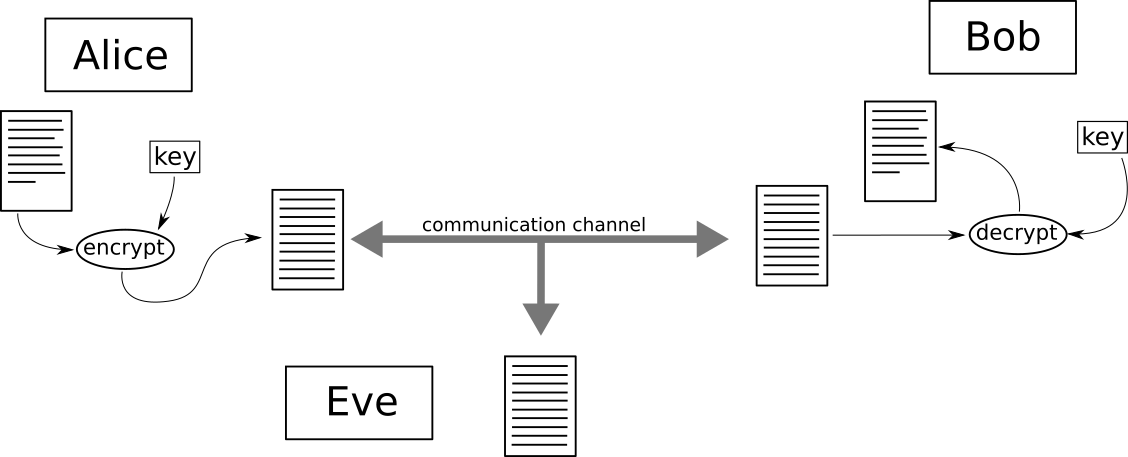
\includegraphics[scale=0.350]{images/symmetric_ecryption.png}
\caption{Alice and Bob symmetrically encrypt and decrypt a message}
\label{}
\end{figure}
While symmetric encryption is the oldest form of encryption, being used for over 4000 years, it does have a major drawback -- the key distribution problem: if Alice and Bob are separate parties (as in the case of secure message transmission), they must exchange their key beforehand using a secure channel \cite{cryptography}.
If an eavesdropper, Eve, were to intercept the key in transit, then the encryption is compromised and there is not necessarily any way for Alice or Bob to know.

% Talk about AES encryption and/or stream cyphers

% One Time Pad in depth
A One-Time-Pad (OTP) is a symmetric key that is used only once.
The OTP, as the name suggests, is discarded after a singe message has been sent, and the OTP is usually the same length as the message it encrypts.
This allows bit-wise encryption techniques, such as parity manipulation, to add the the security of the key and ensures that common frequency hacking techniques are not possible \cite{cryptography}.
In order to make the OTP truly secure, the bits used must be generated using a true-random number generator to avoid a malicious party guessing the pad.
Data is encrypted using a OTP with the following bitwise operation:
\begin{center}
\begin{tabular}{rc}
Plaintext: & $X = \{x_0, x_1, ..., x_n\}$ \\
OTP:  & $P = \{p_0, p_1, ..., p_n\}$  \\
Cyphertext:  & $Y = \{y_0, y_1, ..., y_n \}$\\
where  & $y_i = (x_i + p_i) \mod 2 $\\
\end{tabular}
\end{center}

For example, in binary:

\begin{center}
\begin{tabular}{rc}
Plaintext: &  \code{ 0 1 0 0 1 0 1 0} \\
OTP: &        \code{ 0 1 1 0 1 0 0 1} \\
Cyphertext: & \code{ 0 0 1 0 0 0 1 1} \\
\end{tabular}
\end{center}

To decrypt the cyphertext using the OTP, you simply apply the same opperation:

\begin{center}
\begin{tabular}{rc}
Cyphertext: & \code{ 0 0 1 0 0 0 1 1} \\
OTP: &        \code{ 0 1 1 0 1 0 0 1} \\
Plaintext: &  \code{ 0 1 0 0 1 0 1 0} \\
\end{tabular}
\end{center}
Under the proper conditions, a OTP is considered to be ``perfect encryption", and is only susceptible to brute force attacks, where one has to try every possible combination of the secret key, which is computationally infeasible \cite{cryptography}.
% One Time Pad caveats
However OTPs suffer from the same issue as all symmetric encryption protocols, the key distribution problem.
In the case of the OTP, not only does one encryption key have to be distributed, a unique key must be distributed for each message, making it highly impractical in most cases.

\subsection{Asymmetric Encryption}
% Asymmetric encryption
Asymmetric encryption, also known as public-key cryptography, on a classical computer, is the process of encrypting data using one key in such a way that it can be decrypted using a different key.
In effect, Alice can encrypt a message using a key that is publicly accessible, and the message can only be decrypted by Bob, who has the secret key corresponding to the public key used.
This method requires a key to be compromised of two parts, a public and private key-pair: $k = (k_{pub}, k_{priv})$ where $k_{pub} = f(k_{priv})$ \cite{cryptography}.

% Diffie Hellman in depth
The Diffie-Hellman KEP was the first asymmetric KEP to be proposed, and is still widely used in various forms today. 
It is performed as follows:

\begin{enumerate}
\item The sender and receiver, Alice and Bob respectively, establish a line of communication.
\item Some large prime $p$ and an integer $\alpha \in \{2,3,4,...,p-2\}$ are shared between Alice and Bob.
\item Alice and Bob each compute their own private keys, $a$ and $b$, respectively. $$k_{priv,A} = a \in \{2,3,4,...,p-2\}$$
\item Alice sends Bob her public key $A = \alpha^a \mod p$.
\item Bob sends Alice his public key $B = \alpha^b \mod p$. 
\item Alice computes a session key $k_{AB} = B^a \mod p$.
\item Bob computes a session key $k_{AB} = A^b \mod p$. 
Because $(\alpha^a)^b = (\alpha^b)^a = \alpha^{ab}$, both Alice and Bob's computations result in the same session key despite never knowing each other's private keys. 
\end{enumerate}

This method is cryptographically secure due to the Discreet Logarithm Problem (DLP), finding $x$ such that $B = \alpha^x \mod p$. 
This problem is computationally not feasible to solve using classical computers; although it has never been shown to be NP-Hard, nor has it been shown to be polynomial time solvable \cite{Shor_1997}.
Although these techniques are currently secure, they become easy to solve in the quantum space.

\section{Quantum Computation}

% Basic properties
Just as classical computation involves bits, quantum computation is computation using quantum bits, qubits, which are usually denoted using ``bra-ket" notation as $\ket{\psi}$ \cite{qc:agi}.
A ket is simply a representation of a vector, and in this case the vector is the ``state-vector" of the qubit, as further explained.
Similar to classical bits having the value 0 or 1, qubits' state can be the analogous $\ket{0}$ or $\ket{1}$.
These states will be used as binary, just like 0 and 1, for computation.
%	State
It is commonly said that while a classical bit exists in either the state 0 or 1, qubits can exist in both $\ket{0}$ and $\ket{1}$ at once.
There is an element of truth in this, but a more accurate description would be that as a qubits state-vector exists in a 3-dimensional space, and it can point somewhere in between the states $\ket{0}$ and $\ket{1}$. 
This state-vector is described as a linear combination $\ket{\psi} = \alpha\ket{0} + \beta\ket{1}$, where $|\alpha|^2 + |\beta|^2 = 1$, and $\alpha$ and $\beta$ are referred to as the amplitude of probability for their respective kets.

%	Measurement
Just as a computer can read the value of a classical bit, we can read, or``measure", a qubit.
The measurement is performed against two states, $\ket{0}$ and $\ket{1}$, and upon measurement the qubits state collapses to one of the two values.
The probability with which a vector will collapse into one of two states is the square of the amplitude for that state.
It is unknown exactly what causes the superposition to collapse, but it has been derived from empirical observations and is the single most important property of quantum mechanics \cite{qc:agi}.
For example, consider the qubit $\ket{\psi} = \frac{1}{\sqrt{3}}\ket{0} + \sqrt{\frac{2}{3}}\ket{1}$.
The probability that $\ket{\psi}$ will be $\ket{0}$ when measured is $(\frac{1}{\sqrt{3}})^2$, or $\frac{1}{3}$.
Any qubit or state-vector is defined using this vector formula.
If $\ket{\psi}$ is a linear combination of $\ket{0}$ and $\ket{1}$, and neither amplitudes are zero, the qubit is said to be in a superposition of $\ket{0}$ and $\ket{1}$.
Superposition is one of the fundamental properties of quantum computation \cite{qc:agi}. 

We use quantum operators called gates to manipulate $\alpha$ and $\beta$ probabilities.
For example, the Hadamard Gate, or H gate, performs what is called a "quarter turn"; it maps $$\ket{\psi} = \ket{0} \rightarrow \textSq{H} \rightarrow \ket{\psi} = \frac{1}{\sqrt{2}}\ket{0} + \frac{1}{\sqrt{2}}\ket{1}$$  $$\ket{\psi} = \ket{1} \rightarrow \textSq{H} \rightarrow \ket{\psi} = \frac{1}{\sqrt{2}}\ket{0} - \frac{1}{\sqrt{2}}\ket{1}$$ \cite{qc:agi}.
Since after the H gate is applied $\alpha$ and $\beta$ both equal $\frac{1}{\sqrt{2}}$, and ${(\frac{1}{\sqrt{2}})}^2 = \frac{1}{2}$, if we measure $\ket{\psi}$ in this state it would collapse to $\ket{0}$ and $\ket{1}$ with equal probability. 
It is worth noting this is one way to create a true-random number generator.

%	Bases
Because the state vector exists in a 3D state space, we do not necessarily have to measure against $\ket{0}$ and $\ket{1}$, in fact we can measure against any two vector values that are opposite each other on the unit circle. 
A set of vectors to measure against is known as a basis, and there are many possible bases. 
The set $\{\ket{0},\ket{1}\}$ is known as the standard basis or computational basis, as it is analogous to classical bits \cite{qcftgu}.
Another common basis is the Hadamard Basis, which is denoted $\ket{+} = \frac{1}{\sqrt{2}}\ket{0} + \frac{1}{\sqrt{2}}\ket{1}$ and $\ket{-} = \frac{1}{\sqrt{2}}\ket{0} - \frac{1}{\sqrt{2}}\ket{1}$.
The H gate will put $\ket{0} \rightarrow \ket{+}$ and $\ket{1} \rightarrow \ket{-}$, but it will also revert the Hadamard basis into the standard basis: $\ket{+} \rightarrow \ket{0}$ and $\ket{-} \rightarrow \ket{1}$.

Because the standard basis and the Hadamard basis are perpendicular to each other they are referred to as orthonormal bases.
That is to say if a $\ket{\psi} = \ket{+}$ or $\ket{\psi} = \ket{-}$ then it will have a 50\% change of being $\ket{0}$ or $\ket{1}$ if measured in the standard basis, and vice-versa \cite{qc:agi}. 

\begin{figure}[H]
\centering
\begin{tabular}{cc|cccc}
	&&\multicolumn{4}{|  c }{Measured value}  \\
	   &       &$ \ket{0}$ & $\ket{1}$ & $\ket{+}$ & $\ket{-}$\\ \hline
	\multirow{4}{*}{Qubit state} &$\ket{0}$ & $100\%$   & $0\%$     & $50\%$    &  $50\%$  \\
	&$\ket{1}$ & $0\%$     & $100\%$   & $50\%$    &  $50\%$  \\
	&$\ket{+}$ & $50\%$    & $50\%$    & $100\%$   &  $0\%$   \\
	&$\ket{-}$ & $50\%$    & $50\%$    & $0\%$     &  $100\%$ \\
\end{tabular}
\caption{The probability of measuring a qubit from one basis state into another}
\end{figure}

In effect, if you have a vector in one orthonormal basis it is useless if measured in another orthonormal basis.
Further, since the vector state changes when measured, if a value is encoded in one orthonormal basis, that information is destroyed by measuring in another orthonormal basis \cite{qcftgu}. 

% Guarantees
% 	Copy-ability
Another crucial property of qubits is that they cannot be cloned.
It is impossible to have an operator that clones the state of an input qubit into an output qubit without knowing the basis of the input \cite{qc:agi}.
This property proves crucial in the BB84 protocol, as explained in Chapter~\ref{chap:bb84}.

Using these properties and others, it has been shown that quantum computers can solve the DLP on an $n$-bit number in only $O(n^2\log n \log \log n)$ time \cite{MikeAndIke}.
Therefore, the popularity of quantum computers poses a serious threat to the securities of the Diffie Hellman KEP and asymmetric encryption.
The BB84 protocol is a quantum key distribution (QKD) protocol that allows two parties to co-create a shared key, using a verifiably secure channel, that can then be used to symmetrically encrypt messages.

	    \chapter{Challenges}
\label{chap:challenges}
In the course of developing this serialization framework, numerous challenges were discovered during the background research and testing process. This chapter discusses those challenges. Chapter \ref{chap:framework} discusses the approach that was taken in the design of the serialization framework and the justification for that approach.

\section{Supporting Non IEEE-754 Platforms}
\label{sec:challenges_nonconforming_platforms}
The original goal of this project was to develop a system that would have the ability to completely handle the serialization of floating-point numbers. When developing a portable framework, it is desirable that the end user be able to simply use the framework while minimizing the additional setup required as well as the necessary knowledge regarding the details of their platform. Unfortunately, it quickly became apparent that such a system was implausible.

C++ does not define any requirements for how floating-point numbers are implemented (see Section~\ref{sec:background_cpp}), meaning that it is impossible to predict what floating-point format will be used by a given platform. Most applications developed on desktop/server platforms using x86 or x86-64 processors may be reasonably expected to use IEEE-754. However, C++ compilers are available on a wide variety of system architectures, making it impossible to know in advance all of the different floating-point formats that may be encountered, whether they are implemented with hardware support or via software libraries.

In order to develop a portable framework, the developer must be required to know some information about the system configurations that their software will be used on, so that they may correctly interface with the framework. Serializing floating-point data in a standardized format (see Section~\ref{sec:framework_core}) requires the end user to provide the necessary code to convert the standardized floating-point data into a format compatible with the floating-point types used by their platform. It is also expected that some systems may lack the ability to represent IEEE-754 special values. Infinity and NaN are, after all, a result of the IEEE-754 requirement that computations must always continue, and floating-point formats without that requirement may not have a comparable construct. The framework must therefore have a mechanism to signal when special values are loaded, so that the developer may translate them to an equivalent value or, if unsupported, discard them entirely.

\section{Identifying IEEE-754 Types}
\label{sec:challenges_identifying_types}
It is often necessary to identify the specific type of a floating-point value. ISO C++11 requires the \code{cmath} header of the Standard Library to implement several functions related to floating-point classification \cite{ISO-C++11}. \code{isnormal()}, \code{isnan()}, and \code{isinf()} may be used to determine if their respective parameters are normal numbers, NaN values, or infinity. The function \code{fpclassify()} may also be used; it returns an enumerated value indicating if the parameter is normal, subnormal (denormal), infinity, NaN, or an implementation-defined type that does not match one the IEEE-754 categories. However, it should be noted that the enumerated values returned by \code{fpclassify()} are implementation-defined, meaning that they require additional manipulation before they may be used in a portable manner.

The above functionality is not available when using compilers that do not support the C++11 standard. Prior to C++11, many compilers implemented extensions to their libraries which added functions such as \code{isnan()}, \code{isinf()}, etc. There is no standardized way to detect the presence of these extensions short of manually implementing checks for specific compiler versions. Section~\ref{sec:framework_utilities} describes a set of utility functions that are provided by the framework to assist in the identification of floating-point types.

\section{Not a Number}
\label{sec:challenges_special values}
The bit pattern that IEEE-754 defines to identify NaN values is not fixed (see Section~\ref{subsubsec:nan}). That is, any floating-point value that contains a biased exponent with all bits set and a non-zero fraction field will be recognized as NaN; the necessary bit pattern of the fraction field is not defined by the standard. Additionally, the fraction field of a NaN value may be used to encode implementation-specific data  which may be interpreted differently on various platforms. For example, on one platform a specific bit pattern may represent ``NaN caused by divide by zero.'' If this bit pattern is moved to another platform it will still be interpreted as NaN, however, it may take on a different meaning such as ``NaN caused by $\infty - \infty$.''

Also complicating this problem is the distinction between Quiet and Signaling NaN values. The 2008 update to the IEEE-754 standard addresses this deficiency by requiring that the most significant digit of the fraction string be used to indicate the type of NaN value \cite{IEEE-754-2008}. Some platforms, however, have not yet adopted the updated standard. For example, Microsoft Visual C++ version 12 (Visual Studio 2013) operating on both Windows 7 and Windows 8 generates NaN values that do not conform to the IEEE-754-2008 standard (see Appendix~\ref{app:features}). Since conformance to the 2008 revision of the standard can not be assumed, it is therefore impossible to distinguish between Quiet and Signaling NaN values in a portable manner. As detailed in Section~\ref{sec:framework_core}, the framework will consider all NaN values to be QNaN so that this issue may be avoided.

\section{Size of \code{long double} Values}
\label{sec:challenges_ld_size}
As detailed in Section~\ref{sec:background_ieee754}, the Extended Precision type used to implement \code{long double} is not defined to be a fixed size. There are in fact three common sizes that may be used for \code{long double}: 8, 10, or 16 bytes. The width of the \code{long double} type may vary depending on the available hardware floating-point unit, the operating system, or even on compiler settings.

Conversions between the 10 and 16 byte formats are relatively easy. The two formats are identical except for the width of the fraction field (see Table~\ref{table:fp_types}), therefore a conversion from 10 to 16 bytes may be done by right-padding the fraction field with zeros to the appropriate width, while converting from 16 to 10 bytes requires dropping some bits from the fraction string.

Conversion from the 8 byte format to either 10 or 16 bytes requires modification of the exponent field, as the formats have exponents of differing widths. If the value is normal, the biased exponent must be modified using the formula $E_{b} = E_{b} \pm (b_{\code{long double}} - b_{\code{double}})$, performing addition when the conversion is from 8 bytes to 10/16 bytes, or subtraction when converting from 10/16 to 8 bytes. If the value is denormal, infinity, or NaN, 8 byte to 10/16 byte conversions require the exponent field must be right padded to the correct width by duplicating the least significant digit of the exponent field; conversion from 10/16 byte to 8 byte formats require the exponent field to be trimmed to the correct width. In conversions of all value types, the fraction field must also be modified to the correct width by right-padding or removing extra digits using a round to nearest mode.

An additional problem occurs in some implementations of the 10 byte type. Testing revealed that some implementations (see Appendix~\ref{app:features}) use a 10 byte \code{long double} type that is actually stored in 16 bytes of memory. In these situations \code{sizeof(long double)} will return 16, meaning that \code{sizeof(long double)} alone is insufficient to distinguish between the 10 and 16 byte types. As a solution to this issue, the algorithm shown in Listing~\ref{listing:10in16} was used. This algorithm sets a negative \code{long double} value and detects if the most significant bit is set, as would be expected for a true 16 byte value. Unfortunately testing also showed that some implementations of the 10 byte format using 16 bytes of storage make use of the additional bytes to store implementation-specific data whose purpose is unknown. In the systems observed during testing, the most significant bit of the storage was not used for storing additional information. If, however, an implementation did choose to use the most significant bit for extra information, it would invalidate this solution.

\noindent
\begin{minipage}{\linewidth}
\begin{singlespace}
\begin{lstlisting}[language={}, caption=An algorithm to detect 10 byte values that use 16 bytes of storage., label=listing:10in16]
function detect_10_byte_format_in_16_byte_storage:
    if long double size is not 16 bytes then
        return false
    end if

    set a long double variable to -1
    obtain the most significant bit of the variable
    if the bit is 1 then
        return false
    else
        return true
    end if
\end{lstlisting}
\end{singlespace}
\end{minipage}

\section{x86 Extended Precision Format}
\label{sec:challenges_x86_ext}

\begin{table}
  \centering
  \caption{x86 Extended Precision explicit fraction bits.}
  \label{table:x86_ext_fraction_msb}
  \begin{tabular}{|l|l|}
    \hline
    \textbf{Value Type} & \textbf{Fraction msb} \\
    \hline
    Normal Numbers      & 1                     \\
    \hline
    Denormal Numbers    & 0                     \\
    \hline
    Infinity            & 1                     \\
    \hline
    Not a Number        & 1                     \\
    \hline
  \end{tabular}
\end{table}

Most sources indicate that a 10 byte \code{long double} may be expected to use the standard IEEE-754 format as described in Section \ref{subsec:fp_format}. However, additional research and practical testing determined that many 10 byte types do not strictly conform to the standard. Instead, they use the x86 Extended Precision floating-point format implemented by Intel x87 hardware floating-point units. This format is based on IEEE-754, but differs from the standard by requiring the most significant digit of the fraction to be explicitly encoded in the value as listed in Table~\ref{table:x86_ext_fraction_msb} \cite{Intel:DevManual}. The remainder of the fraction field conforms to the IEEE-754 standard.

The explicitly encoded leading fraction digit causes numerous problems. When one treats x86 Extended Precision values as though they are standard IEEE-754 values, normal and denormal values will be calculated incorrectly because the explicit fraction MSB causes the fraction to be effectively divided by two. Infinity values will always be recognized as NaN due to the non-zero fraction field. Finally, NaN values will always be recognized as QNaN.

Solutions to this issue are not trivial. Some possible approaches to handle this issue are addressed in Chapter~\ref{chap:conclusion}.
      \chapter{Proposed Framework}
\label{chap:framework}
This chapter presents a framework to allow for the portable serialization of floating-point numbers that attempts to address the issues presented in Chapter \ref{chap:challenges}. In addition to the core framework, a number of helper utilities are provided, as well as details regarding integration with the Boost Serialization Library, and an example usage of the framework.

\section{Framework Core}
\label{sec:framework_core}
The framework consists of two major components: a set of standards dictating how floating-point numbers will be serialized, and a pair of abstract base classes that provide the interface for serialization and de-serialization. Users of the framework must implement these interfaces so that the serialization implementation saves floating-point values in a manner compliant with the framework requirements, while the de-serialization implementation loads framework compliant values and converts them to a format compatible with the user's platform.

\subsection{Serialization Standards}
When using this framework, users shall adhere to the following standards to ensure that floating-point values may be saved and loaded in a consistent manner:

\begin{enumerate}
  \item Binary Representation
  \begin{enumerate}
    \item Within the framework, floating-point values shall always be treated as binary values. 
    \begin{enumerate}
      \item The types \code{float}, \code{double}, and \code{long double} shall only be used to obtain the representation when a value enters the framework before serialization, and to set the final floating-point number as the value leaves the framework following de-serialization. In other words, no floating-point instructions or casts are to be used in the serialization or de-serialization code. This ensures that the underlying bit pattern is only changed when desired by the developer.
      
      \item The type \code{uint32\_t} shall be used to hold the binary representation of a \code{float}, and the type \code{uint64\_t} shall be used to hold the binary representation of a \code{double}.
      
      \item Since \code{long double} may vary in size, its binary representation shall be held in 128 bits using a pair of \code{uint64\_t} values. True 128 bit integer types remain uncommon, therefore the choice of \code{uint64\_t[2]} ensures greater portability.
    \end{enumerate}
    
    \item The integer types that hold the binary values shall be serialized using a byte ordering consistent with how the containing serialization library handles integer types. In this thesis, the Boost Serialization Library is used, and integer types are serialized using the built-in functionality of that library.
    
    \item When a \code{long double} is serialized, the integer representing the most significant portion of the binary value shall be written first, followed by the integer representing the least significant portion of the binary value.
  \end{enumerate}
  
  \item Floating-Point Format
  \begin{enumerate}
    \item All values shall be serialized using a bit pattern that represents a value conforming to the appropriate IEEE-754 format. \code{long double} values shall always use the 128 bit Extended Double Precision format.
    
    \item Whenever possible, values shall be serialized as a normal number.
    
    \item Any number that falls within the range of IEEE-754 denormal values shall be serialized using a denormal number representation. Zero always uses a denormal representation.
    
    \item Any number that falls outside the range of IEEE-754 normal values shall be serialized as either $+\infty$ or $-\infty$.
    
    \item All NaN values shall be considered to be QNaN.
    
    \item During de-serialization, an implementation must recognize all denormal, infinity, and NaN values, and convert them to an appropriate format as required by the target floating-point format.
    \begin{enumerate}
      \item If a denormal value is detected during de-serialization and the target floating-point format does not support denormal values or is otherwise incapable of representing the value, the value shall be replaced with the target format's representation of zero.

      \item When a NaN value is detected during de-serialization and the target floating-point format is IEEE-754, it is recommended to replace the loaded binary value with the target system's QNaN representation, obtained using the facilities of the C++ Standard Library\footnote{\code{std::numeric\_limits<T>::quiet\_NaN()}; \code{T} is the floating-point type.}.

      \item If an infinity or NaN value is detected during de-serialization and the target floating-point format is incapable of representing either infinity or NaN, it is recommended to signal an error condition or to raise an exception. If de-serialization is allowed to continue, the value returned in place of infinity or NaN is implementation-defined.
    \end{enumerate}    
  \end{enumerate}
\end{enumerate}

\subsection{Serialization Interface}
The abstract base class (interface) \code{FP\_Serializer}, shown in Listing~\ref{listing:framework_serializer}, provides the means by which the local floating-point type is converted to a binary value suitable for serialization. A serialization library using this framework shall require the user to provide an implementation of the \code{FP\_Serializer} interface before serialization begins.

When the library encounters a floating-point value, it shall call the corresponding \code{convert()} method. The parameter \code{in} shall be the floating-point value to be serialized, passed using the floating-point format of the current platform. The implementation shall set the parameter \code{out} to be the binary value that will be serialized, conforming to the requirements listed above. The library shall then perform serialization of the integer value containing the binary representation stored in \code{out}.

\noindent
\begin{minipage}{\linewidth}
\begin{singlespace}
\begin{lstlisting}[caption=The \code{FP\_Serializer} interface., label=listing:framework_serializer]
class FP_Serializer
{
public:
    virtual ~FP_Serializer() {}
    
    virtual void convert(const float in, uint32_t& out) const = 0;
    virtual void convert(const double in, uint64_t& out) const = 0;
    virtual void convert(const long double in, LongDouble& out) const = 0;
};
\end{lstlisting}
\end{singlespace}
\end{minipage}

\subsection{De-serialization Interface}
The counterpart to \code{FP\_Serializer} is the abstract base class (interface) \code{FP\_Deserializer}, shown in Listing~\ref{listing:framework_deserializer}. It is used to convert the binary value loaded during de-serialization into a suitable floating-point value that is compatible with the current platform. A serialization library using this framework shall require the user to provide an implementation of the \code{FP\_Deserializer} interface before de-serialization begins.

When the library receives a request that a floating-point value be loaded, it shall first de-serialize the appropriate integer type, which will contain the binary representation of the floating-point value. This integer shall then be passed to the appropriate \code{convert()} method as the parameter \code{in}. The \code{convert()} method determines what type of floating-point value the \code{in} parameter represents, and calls the appropriate method to handle the conversion of the loaded type. Four methods are provided for each type: \code{loadedNorm()}, \code{loadedDenorm()}, \code{loadedNan()}, \code{loadedInf()}. Each method takes a single parameter, which is the binary representation of the loaded value, performs a conversion of the binary representation to the appropriate floating-point type. This floating-point value shall then be assigned to the \code{out} parameter of the \code{convert()} method.

Note that it is not strictly necessary to implement all five ``loaded'' methods for each type. For example, the binary representation of a \code{float} specified by this framework may be converted directly to the \code{float} type of a platform that conforms to IEEE-754 (see Section~\ref{sec:framework_example}). However, even in that case it is still recommended to implement \code{loadedNan()}, as previously discussed.

\noindent
\begin{minipage}{\linewidth}
\begin{singlespace}
\begin{lstlisting}[caption=The \code{FP\_Deserializer} interface., label=listing:framework_deserializer]
class FP_Deserializer
{
public:
    virtual ~FP_Deserializer() {}
    
    virtual void convert(const uint32_t in, float& out) const = 0;
    virtual float loadedNorm(const uint32_t v) const = 0;
    virtual float loadedDenorm(const uint32_t v) const = 0;
    virtual float loadedNan(const uint32_t v) const = 0;
    virtual float loadedInf(const uint32_t v) const = 0;
    
    virtual void convert(const uint64_t in, double& out) const = 0;
    virtual double loadedNorm(const uint64_t v) const = 0;
    virtual double loadedDenorm(const uint64_t v) const = 0;
    virtual double loadedNan(const uint64_t v) const = 0;
    virtual double loadedInf(const uint64_t v) const = 0;

    virtual void convert(const LongDouble in, long double& out) const = 0;
    virtual long double loadedNorm(const LongDouble v) const = 0;
    virtual long double loadedDenorm(const LongDouble v) const = 0;
    virtual long double loadedNan(const LongDouble v) const = 0;
    virtual long double loadedInf(const LongDouble v) const = 0;
};
\end{lstlisting}
\end{singlespace}
\end{minipage}

\section{Provided Utilities}
\label{sec:framework_utilities}
To facilitate the identification and conversion of floating-point types within implementations of \code{FP\_Serializer} and \code{FP\_Deserializer}, a set of utility functions and values are provided as part of the framework.

\subsection{Floating-Point Field Masks}
A number of integer constants are supplied that implementations may use when manipulating floating-point numbers as binary values. These constants are shown in Listing~\ref{listing:framework_masks}. Masks are supplied for the 32, 64, and 128 bit types that are used for serialization within the framework. For each type, five constants are provided:

\begin{description}
  \item[\code{biasN} :] The bias for the type, as listed in Table~\ref{table:fp_types}.
  \item[\code{signMaskN} :] A mask that may be used to obtain the sign bit for the type.
  \item[\code{exponentMaskN} :] A mask that may be used to obtain the exponent field for the type.
  \item[\code{fractionMaskN} :] A mask that may be used to obtain the fraction field for the type.
  \item[\code{nanTypeMaskN} :] A mask that may be used to obtain the QNaN/SNaN flag bit if the type conforms to IEEE-754-2008.
\end{description}

In the name of the constant, \code{N} indicates the size of the type, in bits. The 128 bit type actually defines a pair of constants for each item listed above, with \code{hi} or \code{lo} appended to the name, indicating whether that mask applies to the most significant or least significant portion of the value.

\noindent
\begin{minipage}{\linewidth}
\begin{singlespace}
\begin{lstlisting}[caption=Floating-point field masks., label=listing:framework_masks]
const uint32_t bias32 = 127;
const uint32_t signMask32 = UINT32_C(0x80000000);
const uint32_t exponentMask32 = UINT32_C(0x7f800000);
const uint32_t fractionMask32 = UINT32_C(0x007fffff);
const uint32_t nanTypeMask32 = UINT32_C(0x00400000);

const uint64_t bias64 = 1023;
const uint64_t signMask64 = UINT64_C(0x8000000000000000);
const uint64_t exponentMask64 = UINT64_C(0x7ff0000000000000);
const uint64_t fractionMask64 = UINT64_C(0x000fffffffffffff);
const uint64_t nanTypeMask64 = UINT64_C(0x0008000000000000);

const uint64_t bias128 = 16383;
const uint64_t signMask128hi = UINT64_C(0x8000000000000000);
const uint64_t signMask128lo = UINT64_C(0);
const uint64_t exponentMask128hi = UINT64_C(0x7fff000000000000);
const uint64_t exponentMask128lo = UINT64_C(0);
const uint64_t fractionMask128hi = UINT64_C(0x0000ffffffffffff);
const uint64_t fractionMask128lo = UINT64_C(0xffffffffffffffff);
const uint64_t nanTypeMask128hi = UINT64_C(0x0000800000000000);
const uint64_t nanTypeMask128lo = UINT64_C(0);
\end{lstlisting}
\end{singlespace}
\end{minipage}

\subsection{Floating-Point Type Functions}
As discussed in Section~\ref{sec:challenges_identifying_types}, the C++ Standard Library has only recently added functionality to identify the various types of floating-point values. Therefore, the framework includes a selection of utility functions for identifying floating-point values. These functions are intended to be used with binary values within the framework, therefore all of them take the binary representation of the floating-point value as an integer parameter. The following functions are included, with overloads supplied for the each of the 32, 64, and 128 bit floating-point types:

\begin{description}
  \item[\code{isNeg()} :] Returns true if the value is negative, regardless of its type.
  \item[\code{isDenormal()} :] Returns true if the value is a denormal number.
  \item[\code{isNormal()} :] Returns true if the value is a normal number.
  \item[\code{isZero()} :] Returns true if the value is either $+0$ or $-0$.
  \item[\code{isPosZero()} :] Returns true only if the value is $+0$.
  \item[\code{isNegZero()} :] Returns true only if the value is $-0$.
  \item[\code{isInf()} :] Returns true if the value is either $+\infty$ or $-\infty$.
  \item[\code{isPosInf()} :] Returns true only if the value is $+\infty$.
  \item[\code{isNegInf()} :] Returns true only if the value is $-\infty$.
  \item[\code{isNaN()} :] Returns true if the value is Not a Number. Does not distinguish between Quiet or Signaling NaN.
\end{description}

Listing~\ref{listing:framework_type_funcs} contains the prototypes for the included utility functions.

\noindent
\begin{minipage}{\linewidth}
\begin{singlespace}
\begin{lstlisting}[caption=Floating-point type utility functions., label=listing:framework_type_funcs]
bool isNeg(const uint32_t v);
bool isNeg(const uint64_t v);
bool isNeg(const LongDouble v);

bool isDenormal(const uint32_t v);
bool isDenormal(const uint64_t v);
bool isDenormal(const LongDouble v);

bool isNormal(const uint32_t v);
bool isNormal(const uint64_t v);
bool isNormal(const LongDouble v);

bool isZero(const uint32_t v);
bool isZero(const uint64_t v);
bool isZero(const LongDouble v);

bool isPosZero(const uint32_t v);
bool isPosZero(const uint64_t v);
bool isPosZero(const LongDouble v);

bool isNegZero(const uint32_t v);
bool isNegZero(const uint64_t v);
bool isNegZero(const LongDouble v);

bool isInf(const uint32_t v);
bool isInf(const uint64_t v);
bool isInf(const LongDouble v);

bool isPosInf(const uint32_t v);
bool isPosInf(const uint64_t v);
bool isPosInf(const LongDouble v);

bool isNegInf(const uint32_t v);
bool isNegInf(const uint64_t v);
bool isNegInf(const LongDouble v);

bool isNaN(const uint32_t v);
bool isNaN(const uint64_t v);
bool isNaN(const LongDouble v);
\end{lstlisting}
\end{singlespace}
\end{minipage}

\subsection{\code{LongDouble} Type}
\code{long double} may vary in width from 64 to 128 bits, as discussed in Section~\ref{sec:challenges_ld_size}. At this time, integers larger than 64 bits are not commonly available. Therefore, the \code{LongDouble} union type shown in Listing~\ref{listing:framework_longdouble} is provided for ease of accessing the binary representation of a \code{long double} number, as well as converting a binary value back to a \code{long double} type. Within the framework, \code{LongDouble} is always used to encapsulate the pair of \code{uint64\_t} values that hold the binary representation of a \code{long double}. The individual bytes of the type are also accessible, if needed.

Note that on big-endian systems, the integer \code{LongDouble::u64[0]} will refer to the most significant portion of the \code{long double} value, while on little-endian systems it will refer to the least significant portion of the value.

\noindent
\begin{minipage}{\linewidth}
\begin{singlespace}
\begin{lstlisting}[caption=The \code{LongDouble} type., label=listing:framework_longdouble]
union LongDouble
{
    long double ld;
    uint8_t u8[16];
    uint64_t u64[2];
};
\end{lstlisting}
\end{singlespace}
\end{minipage}

\subsection{System Endianness Identification}
Ideally all endianness concerns would be delegated to the containing serialization library. However, as indicated in the previous section, when dealing with the binary representation of \code{long double} values it is necessary for the developer to be aware of the endianness of the current system. The framework provides a utility function, shown in Listing~\ref{listing:framework_endian}, to detect the endianness of the platform.

\noindent
\begin{minipage}{\linewidth}
\begin{singlespace}
\begin{lstlisting}[caption=The endianness identifier utility function., label=listing:framework_endian]
bool isLittleEndian()
{
    union
    {
        uint16_t u16;
        uint8_t u8[2];
    } endian;

    endian.u16 = 0x1234;
    return endian.u8[0] == 0x34;
}
\end{lstlisting}
\end{singlespace}
\end{minipage}

\subsection{\code{long double} Type Identifier.}
As discussed in Section~\ref{sec:challenges_ld_size}, 10 byte \code{long double} values may be stored using 16 bytes of memory. The framework includes a utility function to address this issue, shown in Listing~\ref{listing:framework_ldtype}. This is an implementation of the algorithm from Listing~\ref{listing:10in16}.

\noindent
\begin{minipage}{\linewidth}
\begin{singlespace}
\begin{lstlisting}[caption=The \code{long double} type identifier utility function., label=listing:framework_ldtype]
bool LDis10in16()
{
    if (sizeof(long double) != 16)
        return false;

    LongDouble ld = { -1.0L };
    if (isLittleEndian())
        return !(ld.u64[1] & signMask128hi);
    else
        return !(ld.u64[0] & signMask128hi);
}
\end{lstlisting}
\end{singlespace}
\end{minipage}

\section{Integration With Boost the Serialization Library}
\label{sec:framework_integration}
The Boost Serialization Library, discussed in Section~\ref{sec:background_boost}, is the serialization library used for testing the framework in this thesis. The example \code{Archive} classes provided with the library are \code{portable\_binary\_oarchive}, used for serialization, and \code{portable\_binary\_iarchive}, used for de-serialization. In order to accommodate this floating-point framework, these classes were modified as follows:

\begin{enumerate}
  \item Addition of the floating-point interfaces.
  \begin{enumerate}
    \item A protected member was added to \code{portable\_binary\_oarchive}, which is used to hold an implementation of the \code{FP\_Serializer} interface.
    \item A protected member was added to \code{portable\_binary\_iarchive}, which is used to hold an implementation of the \code{FP\_Deserializer} interface.
  \end{enumerate}
  
  \item Each class was modified so that the methods that perform floating-point serialization function as described in Section~\ref{sec:framework_core}.
\end{enumerate}

Listing~\ref{listing:framework_boost_oarchive} and Listing~\ref{listing:framework_boost_iarchive} show the changes made to these classes.

\noindent
\begin{minipage}{\linewidth}
\begin{singlespace}
\begin{lstlisting}[caption=Modifications to the \code{portable\_binary\_oarchive} class., label=listing:framework_boost_oarchive]
class portable_binary_oarchive
{
protected:
    FP_Serializer& m_fp_serializer;    
public:
    void save(const float& t)
    {
        uint32_t v;
        this->m_fp_serializer.convert(t, v);
        this->primitive_base_t::save(v);
    }
    void save(const double& t)
    {
        uint64_t v;
        this->m_fp_serializer.convert(t, v);
        this->primitive_base_t::save(v);
    }
    void save(const long double& t)
    {
        LongDouble out;
        this->m_fp_serializer.convert(t, out);
        this->primitive_base_t::save(out.u64[0]);
        this->primitive_base_t::save(out.u64[1]);
    }
};
\end{lstlisting}
\end{singlespace}
\end{minipage}

\noindent
\begin{minipage}{\linewidth}
\begin{singlespace}
\begin{lstlisting}[caption=Modifications to the \code{portable\_binary\_iarchive} class., label=listing:framework_boost_iarchive]
class portable_binary_iarchive
{
protected:
    FP_Deserializer& m_fp_deserializer;    
public:
    void load(float& t){
        uint32_t v;
        this->primitive_base_t::load(v);
        this->m_fp_deserializer.convert(v, t);
    }    
    void load(double& t){
        uint64_t v;
        this->primitive_base_t::load(v);
        this->m_fp_deserializer.convert(v, t);
    }    
    void load(long double& t)
    {
        LongDouble in;
        this->primitive_base_t::load(in.u64[0]);
        this->primitive_base_t::load(in.u64[1]);
        this->m_fp_deserializer.convert(in, t);
    }
};
\end{lstlisting}
\end{singlespace}
\end{minipage}

\section{Example Usage on IEEE-754 platforms}
\label{sec:framework_example}
To demonstrate the usage of this floating-point framework, an example implementation has been provided that operates on systems supporting IEEE-754. This implementation supports only true IEEE-754 platforms; specifically, platforms that use the x86 Extended Precision type (see Section~\ref{sec:challenges_x86_ext}) are not supported.

Listing~\ref{listing:framework_ieee_serializer} shows the implementation of the \code{FP\_Serializer} interface. In this implementation, \code{float} and \code{double} types are both serialized directly, as their formats are already compliant with the requirements listed in Section~\ref{sec:framework_core}. \code{long double} types are modified to conform to the framework specifications by modifying the binary representation as described in Section~\ref{sec:challenges_ld_size}.

\begin{singlespace}
	\lstinputlisting[label=listing:framework_ieee_serializer, caption=The \code{IEEE754Serializer} class.]{code/ieee754serializer.h}
\end{singlespace}

Listing~\ref{listing:framework_ieee_deserializer} shows the implementation of the \code{FP\_Deserializer} interface. In this implementation, the binary values loaded for \code{float} and \code{double} types are converted directly to their respective floating-point types. \code{long double} values are modified as described in Section~\ref{sec:challenges_ld_size} to match the size of that type on the current platform.

\begin{singlespace}
	\lstinputlisting[label=listing:framework_ieee_deserializer, caption=The \code{IEEE754Deserializer} class.]{code/ieee754deserializer.h}
\end{singlespace}

      \chapter{Testing}
\label{chap:testing}
In order to show the viability of the framework presented in this thesis, a number of tests were performed on both the framework utilities and the framework itself. This section details the methodology used in those tests and their results.

\section{Utilities}
\label{sec:testing_utilities}
The utility functions detailed in Section~\ref{sec:framework_utilities} were tested using several different methods.

The functions \code{isLittleEndian()} and \code{LDis10in16()} were not considered viable for automated testing due to the nature of the information they retrieve. \code{isLittleEndian()} was used during the generation of the floating-point feature reports listed in Appendix~\ref{app:features}, and the output was compared against the known endianness of the processors used in those systems. \code{LDis10in16()} was run on the test systems and the results were manually compared to the \code{long double} values that were also generated as part of the feature reports.

Unit tests were created for the floating-point type identification functions using the Boost Test Library\footnote{\url{http://www.boost.org/doc/libs/1_55_0/libs/test/doc/html/index.html}}. In each test case, at least one valid value was tested along with invalid values from all of the applicable floating-point types. Since all of the testing platforms used IEEE-754 as their native floating-point format, test values were cast directly to their binary representation from the \code{float} and \code{double} types. None of the available test platforms used the 128 bit \code{long double} format, so those version of the utility functions were not included in this test.

Listing~\ref{listing:testing_isneg} demonstrates the test cases for the 32 and 64 bit versions of the \code{isNeg()} utility function. Each function is first tested with a valid negative value. It is then tested with a series of invalid values: a positive number, zero, infinity, and NaN.

\noindent
\begin{minipage}{\linewidth}
\begin{singlespace}
\begin{lstlisting}[caption=Testing the \code{isNeg()} function., label=listing:testing_isneg]
#define BINARY_F(val) \
    do { f = val; fb = *reinterpret_cast<uint32_t*>(&f); } while (0)

#define BINARY_D(val) \
    do { d = val; db = *reinterpret_cast<uint64_t*>(&d); } while (0)

BOOST_AUTO_TEST_CASE(test_isNeg32)
{
    float f;
    uint32_t fb;
    
    // valid values
    BINARY_F(-1.0f);
    BOOST_CHECK(isNeg(fb));
    
    // invalid values
    BINARY_F(1.0f);
    BOOST_CHECK(!isNeg(fb));
    BINARY_F(0.0f);
    BOOST_CHECK(!isNeg(fb));
    BINARY_F(numeric_limits<float>::infinity());
    BOOST_CHECK(!isNeg(fb));
    BINARY_F(numeric_limits<float>::quiet_NaN());
    BOOST_CHECK(!isNeg(fb));
}

BOOST_AUTO_TEST_CASE(test_isNeg64)
{
    double d;
    uint64_t db;
    
    // valid values
    BINARY_D(-1.0);
    BOOST_CHECK(isNeg(db));
    
    // invalid values
    BINARY_D(1.0);
    BOOST_CHECK(!isNeg(db));
    BINARY_D(0.0);
    BOOST_CHECK(!isNeg(db));
    BINARY_D(numeric_limits<double>::infinity());
    BOOST_CHECK(!isNeg(db));
    BINARY_D(numeric_limits<double>::quiet_NaN());
    BOOST_CHECK(!isNeg(db));
}
\end{lstlisting}
\end{singlespace}
\end{minipage}

\section{Framework Implementation}
\label{sec:testing_framework}
The IEEE-754 implementation of the framework, detailed in Section~\ref{sec:framework_example}, was tested on the systems listed in Appendix~\ref{app:features}. Listing~\ref{listing:testing_framework} shows a sample test program, in which a simple \code{struct} containing several floating-point numbers may be serialized or de-serialized. The serialization output was created using Windows, Linux, and Mac OS. Each file was then loaded on the other two platforms and the loaded values were compared to the original values, using both a debugger and standard output. Test programs on all platforms were compiled using version 1.55.0 of the Boost Libraries.

\begin{singlespace}
  \lstinputlisting[label=listing:testing_framework, caption=Testing the framework.]{code/test.cpp}
\end{singlespace}

\subsection{Boost Serialization Issues}
Testing revealed several undocumented issues with the portability of files created using the example \code{portable\_binary\_archive} classes supplied with the Boost Serialization Library. These issues appear to be related to the internal versioning information used by the archive classes; there was no indication that they are directly related to the floating-point framework presented in this thesis. However, the issues are documented because they required manual modification of the serialization output so that testing could be completed.

Initial testing found that files created on Linux platforms would load on Windows platforms, however, when attempting to open a file created on Windows using a Linux platform, the Boost Serialization Library would fail to open the file, throwing an exception indicating that the file version was unsupported. Examination of the two files using a hex editor revealed that the first 0x18 bytes of the files were identical. The first difference in the file occurred at offset 0x19; in the file created using Windows the byte at this offset contained the value 0x0B, while the file created on Linux had the value 0x0A. Editing the Windows file so that offset 0x19 had the value 0x0A allowed the file to be loaded on both Windows and Linux. This problem was consistent regardless of the actual data being serialized, therefore, all files created using Windows were manually edited to change the byte at offset 0x19 to the value 0x0A.

A similar problem was discovered when attempting to load files created on Windows using Mac OS; loading of test files failed with an exception reporting an input stream error. The Windows file was compared to a file generated using Mac OS using a hex editor; however, a consistent fix for this problem was not found because the cause of the error could not be determined conclusively.

\subsection{Testing Results}
\code{float} and \code{double} values were found to de-serialize accurately on all tested platforms. This is expected, as all of the available test systems use IEEE-754 conforming \code{float} and \code{double} representations that did not require modification during serialization.

\code{long double} values presented mixed results. \code{long double} values were successfully de-serialized on similar platforms. Test files created on Windows would de-serialize accurately on Windows, but would de-serialize inaccurately on Linux. Meanwhile, test files created using Linux or Mac OS would de-serialize accurately on those platforms, but would be inaccurate following de-serialization on Windows. It was at this time that additional research was conducted and the x86 Extended Precision format was discovered. It was determined that the explicit leading fraction bit used by that format was the cause of the inaccurate values, as described in Section~\ref{sec:challenges_x86_ext}. Additional attempts were made to modify the implementation to support this format seamlessly alongside the standard IEEE-754 format; however, this was unsuccessful. A separate implementation will be required for systems that use the x86 Extended Precision format.

Ultimately, this testing demonstrates that the framework is conceptually sound. The successful serialization and de-serialization of these values, requires the conversion of the local floating-point format to the standardized format. De-serialization requires that the process be reversed. While this process could not be shown while moving between platforms due to the limitations described above, even serialization and de-serialization on the same platform involved a conversion that is fundamentally the same as the conversion used when de-serializing on another platform.
      \chapter{Conclusion}
\label{chap:conclusion}

\section{Future Work}
At this time, the IEEE-754 implementation is essentially complete for \code{float} and \code{double} values. Developers wishing to support cross-platform serialization of only those types may do so with minimal additional work. Support for \code{long double} values, however, is more complex.

Two primary issues affect the serialization of \code{long double} values. First, the detection of 10 byte \code{long double} values that are stored in 16 bytes of memory is somewhat frail. The algorithm proposed in Section~\ref{sec:challenges_ld_size} and implemented in Section~\ref{sec:framework_utilities} relies on the assumption that these implementations to not use the most significant bit of the storage for implementation-specific information. All of the systems tested as part of this thesis did not use that bit; however, implementations are free to use this space for whatever purpose it wishes. By definition, the extra six bytes of the memory location are not part of the IEEE-754 standard. An alternative mechanism of detecting this format would make the framework more robust.

The second issue is support for systems using the x86 Extended Precision format for \code{long double} values. Ideally a system should be implemented so that the usage of this type may be detected dynamically at runtime. The usage of this type is tied to the Intel x87 Hardware Floating-Point Unit. The x86 processor architecture provides the CPUID instruction, which may be used to query for the presence of an x87 FPU \cite{AMD:CPUID}. However, the physical presence of a FPU does not mean that the operating system and/or compiler has chosen to implement the x86 Extended Precision format. For example, a Lenovo X220 laptop was used to provide two of the testing platforms in this thesis. This laptop uses an Intel Core i7 Mobile processor, which includes an x87 FPU\footnote{\url{http://www.intel.com/content/www/us/en/processors/core/CoreTechnicalResources.html}}. When running the Windows operating system, \code{long double} is aliased to \code{double}; when using Linux, the x86 Extended Precision format is used. It seems unlikely that the CPUID instruction alone would be sufficient to detect this format, but perhaps that runtime information could be combined with compile time detection of common operating systems and compilers.

Additional work also remains to be done by implementing the framework for platforms that do not use some form of the IEEE-754 standard.

\section{Summary}
The framework described in this thesis lays the groundwork that developers may use to allow for the serialization of floating-point numbers in a portable manner.

Floating-point numbers that are serialized using this framework are saved to a standard format based on the IEEE-754 floating-point standard. This allows these values to be more easily converted into the format used by a specific target platform. Presented along with the framework is an implementation that supports serialization and de-serialization of floating-point numbers on platforms that support the IEEE-754 standard. In addition, numerous utility functions are provided to assist developers in creating additional implementations.

The variations in floating-point format mean that compromises are inherit in any serialization system. This framework minimizes those compromises by avoiding loss of precision, unless it is required by the target system, as well as maintaining IEEE-754 special values throughout the serialization process.
		\end{doublespace}

	\newpage
    \newlinestretch{1}
	\addcontentsline{toc}{chapter}{Bibliography}
    \bibliographystyle{plain}
	\bibliography{bibliography}
    \nocite{*}
    \begin{appendices}
      \begin{singlespace}
        \chapter{Floating-Point Feature Tests}
\label{app:features}
During the research for this thesis a number of computers and operating systems were tested to determine the floating-point features of each platform. System information was queried in the following manner:

\begin{description}
  \item[Windows:] Operating system and version as well as CPU model number was taken from the ``System Information'' application.
  \item[Mac OS X:] Operating system and version as well as CPU model number was taken from the ``About This Mac'' dialog.
  \item[Linux:] Operating system and version was determined by running the terminal command \code{cat~/etc/*-release}. CPU model number was taken from the file \code{/proc/cpuinfo}.
\end{description}

All other information regarding floating-point features was determined by querying the \code{std::numeric\_limits} class that is included in the C++ Standard Library.

\newpage
\lstinputlisting[caption=Floating-point features of Windows 7., language={}, frame={}, numbers={none}]{reports/laptop_windows.txt}

\newpage
\lstinputlisting[caption=Floating-point features of Windows 8., language={}, frame={}, numbers={none}]{reports/tss_desktop.txt}

\newpage
\lstinputlisting[caption=Floating-point features of Mac OS X., language={}, frame={}, numbers={none}]{reports/tss_imac.txt}

\newpage
\lstinputlisting[caption=Floating-point features of Manjaro Linux on a virtual machine., language={}, frame={}, numbers={none}]{reports/laptop_linux_vm.txt}

\newpage
\lstinputlisting[caption=Floating-point features of CentOS Linux., language={}, frame={}, numbers={none}]{reports/pub2.txt}

\newpage
\lstinputlisting[caption=Floating-point features of Red Hat Linux., language={}, frame={}, numbers={none}]{reports/student.txt}
      \end{singlespace}    
    \end{appendices}
\end{document}
